\documentclass[t]{beamer}
\usefonttheme{serif}
\usetheme[white]{Wisconsin}
\title{Research Update}
%\subtitle{}
\author{Lucas Jacobson}
\institute{University of Wisconsin--Madison}
\date{30 August 2019}

\usepackage{amsmath}
\usepackage{textcomp}

\newcommand{\tildecenter}{\raisebox{0.5ex}{\texttildelow}}

\begin{document}

% ==============================================================================
% Title page
% ==============================================================================

\begin{frame}
  \titlepage
\end{frame}

% ==============================================================================
% Introduction
% ==============================================================================

\begin{frame}
  \frametitle{Research Aims}
  \textbf{Using a novel methodology, create a toolset that can be used to
  automate the optimization of geometry to achieve specific objectives derived
  from nuclear responses.}
  \newline\newline
  Here is the current plan for how this will be done:
  \begin{enumerate}[1]
    \item Use perturbation theory to develop a perturbed version of the neutron
          transport equation in which the perturbation in the detector response
          can be expressed in terms of a material or geometry perturbation.
    \item Use a deterministic radiation transport code to calculate the
          quantities necessary to calculate the perturbation in the detector
          response.
    \item Use shape optimization methods to iteratively alter the geometry in
          order to guide it towards the most optimal configuration.
  \end{enumerate}
\end{frame}

% ==============================================================================
% Math section
% ==============================================================================

\begin{frame}
  \frametitle{Transport Equation}
  \begin{itemize}
    \item The time-independent transport equation is a balance between particles
          leaving a region of phase space and particles entering it.
  \end{itemize}
  \vskip-0.1in
  \begin{multline}
    \hat{\Omega}\cdot\vec{\nabla}\psi\left(\vec{r},\hat{\Omega},E\right) +
    \sigma_t\left(\vec{r},E\right)\psi\left(\vec{r},\hat{\Omega},E\right) - \\
    \iint\sigma_s\left(\vec{r},\hat{\Omega}^\prime\rightarrow\hat{\Omega},E^\prime\rightarrow E\right)\psi\left(\vec{r},\hat{\Omega}^\prime,E^\prime\right)d\hat{\Omega}^\prime dE^\prime =
    q\left(\vec{r},\hat{\Omega},E\right)
  \end{multline}
  \vskip-0.1in
  \begin{scriptsize}\begin{itemize}
    \item Independent variable: angular flux
          $\psi\left(\vec{r},\hat{\Omega},E\right)$
    \item Total cross section:
          $\sigma_t\left(\vec{r},E\right)$
    \item Scattering cross section:
          $\sigma_s\left(\vec{r},\hat{\Omega}^\prime\rightarrow\hat{\Omega},E^\prime\rightarrow E\right)$
    \item Net removal due to streaming:
          $\hat{\Omega}\cdot\vec{\nabla}\psi$
    \item Removal due to collision:
          $\sigma_t\psi$
    \item Net gain due to scattering:
          $\iint\sigma_s\psi d\hat{\Omega}^\prime dE^\prime$
    \item Gain due to external sources:
          $q$
  \end{itemize}\end{scriptsize}
  In operator notation:
  \begin{equation}
    H\psi = q
  \end{equation}
\end{frame}

\begin{frame}
  \frametitle{Adjoint Transport Equation}
  \begin{multline}
    -\hat{\Omega}\cdot\vec{\nabla}\psi^+\left(\vec{r},\hat{\Omega},E\right) +
    \sigma_t\left(\vec{r},E\right)\psi^+\left(\vec{r},\hat{\Omega},E\right) - \\
    \iint\sigma_s\left(\vec{r},\hat{\Omega}\rightarrow\hat{\Omega}^\prime,E\rightarrow E^\prime\right)\psi^+\left(\vec{r},\hat{\Omega}^\prime,E^\prime\right)d\hat{\Omega}^\prime dE^\prime =
    q^+\left(\vec{r},\hat{\Omega},E\right)
  \end{multline}
  \begin{itemize}
    \item The adjoint flux $\psi^+$ in a region of phase space is the importance
          of that region of phase space to the detector $q^+$.
    \item In the adjoint system, particles stream outwards from the detector and
          gain energy when they scatter.
  \end{itemize}
  In operator notation:
  \begin{equation}
    H^+\psi^+ = q^+
  \end{equation}
  Adjoint identity (from the definition of the adjoint):
  \begin{equation}
    \left<\psi,q^+\right> = \left<\psi^+,q\right>
  \end{equation}
\end{frame}

\begin{frame}
  \frametitle{Perturbations}
  \begin{itemize}
    \item Small perturbations in the cross sections result in small
          perturbations in the angular flux.
    \item Notation: perturbed values are written as $\bar{x}$, and
          the perturbation in values are written as $\delta x$.
  \end{itemize}
  Perturbed total cross section:
  \begin{equation}
    \bar{\sigma}_t\left(\vec{r},E\right) \equiv
    \sigma_t\left(\vec{r},E\right) +
    \delta\sigma_t\left(\vec{r},E\right)
  \end{equation}
  Perturbed scattering cross section:
  \begin{multline}
    \bar{\sigma}_s\left(\vec{r},\hat{\Omega}\rightarrow\hat{\Omega}^\prime,E\rightarrow E^\prime\right) \equiv \\
    \sigma_s\left(\vec{r},\hat{\Omega}\rightarrow\hat{\Omega}^\prime,E\rightarrow E^\prime\right) +
    \delta\sigma_s\left(\vec{r},\hat{\Omega}\rightarrow\hat{\Omega}^\prime,E\rightarrow E^\prime\right)
  \end{multline}
  Angular flux in the perturbed system:
  \begin{equation}
    \bar{\psi}\left(\vec{r},\hat{\Omega},E\right) \equiv
    \psi\left(\vec{r},\hat{\Omega},E\right) +
    \delta\psi\left(\vec{r},\hat{\Omega},E\right)
  \end{equation}
\end{frame}

\begin{frame}
  \frametitle{Perturbed Transport Equation}
  Transport equation repeated:
  \begin{equation*}
    \hat{\Omega}\cdot\vec{\nabla}\psi +
    \sigma_t\psi -
    \iint\sigma_s\psi d\hat{\Omega}^\prime dE^\prime =
    q
  \end{equation*}
  Transport equation in the perturbed system:
  \begin{equation}
    \hat{\Omega}\cdot\vec{\nabla}\bar{\psi} +
    \bar{\sigma}_t\bar{\psi} -
    \iint\bar{\sigma}_s\bar{\psi} d\hat{\Omega}^\prime dE^\prime =
    q
  \end{equation}
  \begin{equation}
    \hat{\Omega}\cdot\vec{\nabla}\left(\psi + \delta\psi\right) +
    \left(\sigma_t + \delta\sigma_t\right)\left(\psi + \delta\psi\right) -
    \iint\left(\sigma_s + \delta\sigma_s\right)\left(\psi + \delta\psi\right)d\hat{\Omega}^\prime dE^\prime =
    q
  \end{equation}
  Subtract the original transport equation:
  \begin{multline}
    \hat{\Omega}\cdot\vec{\nabla}\delta\psi +
    \left(\sigma_t\delta\psi + \delta\sigma_t\psi + \delta\sigma_t\delta\psi\right) - \\
    \iint\left(\sigma_s\delta\psi + \delta\sigma_s\psi + \delta\sigma_s\delta\psi\right)d\hat{\Omega}^\prime dE^\prime =
    0
  \end{multline}
\end{frame}

\begin{frame}
  \frametitle{Perturbed Transport Equation (Continued)}
  In perturbation theory it is common to discard the second-order terms:
  \begin{equation}
    \hat{\Omega}\cdot\vec{\nabla}\delta\psi +
    \left(\sigma_t\delta\psi + \delta\sigma_t\psi\right) -
    \iint\left(\sigma_s\delta\psi + \delta\sigma_s\psi\right)d\hat{\Omega}^\prime dE^\prime =
    0
  \end{equation}
  Finally, after rearranging terms:
  \begin{equation}
    \hat{\Omega}\cdot\vec{\nabla}\delta\psi +
    \sigma_t\delta\psi -
    \iint\sigma_s\delta\psi d\hat{\Omega}^\prime dE^\prime =
    \iint\delta\sigma_s\psi d\hat{\Omega}^\prime dE^\prime - \delta\sigma_t\psi
  \end{equation}
  The perturbed transport equation looks very similar to the original transport
  equation: \textbf{the perturbation in the angular flux can be calculated by
  solving the transport equation with the unperturbed cross sections and with an
  external source equal to
  $\iint\delta\sigma_s\psi d\hat{\Omega}^\prime dE^\prime - \delta\sigma_t\psi$.}

  In operator notation:
  \begin{equation}
    H\delta\psi = -\delta H\psi
  \end{equation}
\end{frame}

\begin{frame}
  \frametitle{Perturbed Detector Response}
  Unperturbed detector response:
  \begin{equation}
    R = \left<\psi,q^+\right> = \left<\psi^+,q\right>
  \end{equation}
  Perturbed detector response:
  \begin{equation}
    \bar{R} = \left<\bar{\psi},q^+\right> = \left<\bar{\psi}^+,q\right>
  \end{equation}
  Perturbation in the detector response:
  \begin{equation}\begin{split}
    \delta R & = \bar{R} - R \\
             & = \left<\bar{\psi},q^+\right> - \left<\psi,q^+\right> \\
             & = \left<\delta\psi,q^+\right> \\
             & \stackrel{
\includegraphics[height=\fontcharht\font`\B]{thinking-face.png}}{=}
               \left<\psi^+,-\delta H\psi\right>
  \end{split}\end{equation}
\end{frame}

\begin{frame}
  \frametitle{Math Summary}
  \begin{equation*}
    \delta R = \left<\psi^+,-\delta H\psi\right>
  \end{equation*}
  \begin{itemize}
    \item If $\psi$ and $\psi^+$ are known, then $\delta R$ can be calculated
          for any number of perturbations.
    \item Thus, $\psi$ and $\psi^+$ only need to be calculated once in order to
          be able to calculate the effects of making a perturbation anywhere in
          the entire geometry.
  \end{itemize}
\end{frame}

% ==============================================================================
% Implementation section
% ==============================================================================

\begin{frame}
  \frametitle{ADVANTG}
  \begin{itemize}
    \item ADVANTG -- AutomateD VAriaNce reducTion Generator
    \item Was mainly developed to provide users with MCNP weight windows using
          the CADIS and FW-CADIS methodologies
    \item Uses the 3D discrete ordinates deterministic radiation transport code
          Denovo under the hood
    \item Provides a very convenient way for users to run forward and adjoint
          deterministic transport on MCNP models (no need to use its weight
          window-producing capability)
    \item Has a very convenient undocumented feature which writes the full
          5-dimensional $(E,z,y,x,\hat{\Omega})$ forward and adjoint angular
          fluxes to HDF5 files
  \end{itemize}
\end{frame}

\begin{frame}
  \frametitle{ADVANTG Implementation}
  \begin{itemize}
    \item ADVANTG can be configured to provide most of the information needed to
          calculate $\delta R$, but not all of it, so the Python source code
          needed to be modified to have it output this additional information.
    \item The calculation of $\delta R$ takes place outside ADVANTG. This code
          was originally written in Python, but it was rewritten in C++ because
          it was far too slow.
    \item The following slides show the results for a simple test problem.
  \end{itemize}
\end{frame}

% ==============================================================================
% Test problem section
% ==============================================================================

\begin{frame}
  \frametitle{Test Problem Overview}
  \vskip-0.35in
  \begin{columns}
    \column{0.35\textwidth}
    \begin{itemize}
      \vskip 0.1in
      \item At Phoenix, I was given the task to model one of Phoenix's DD
            solid-target neutron generators and maximize the ${}^{235}\text{U}$
            fission rate in a region behind a thin iron wall.
    \end{itemize}
    \column{0.65\textwidth}
    \begin{figure}
      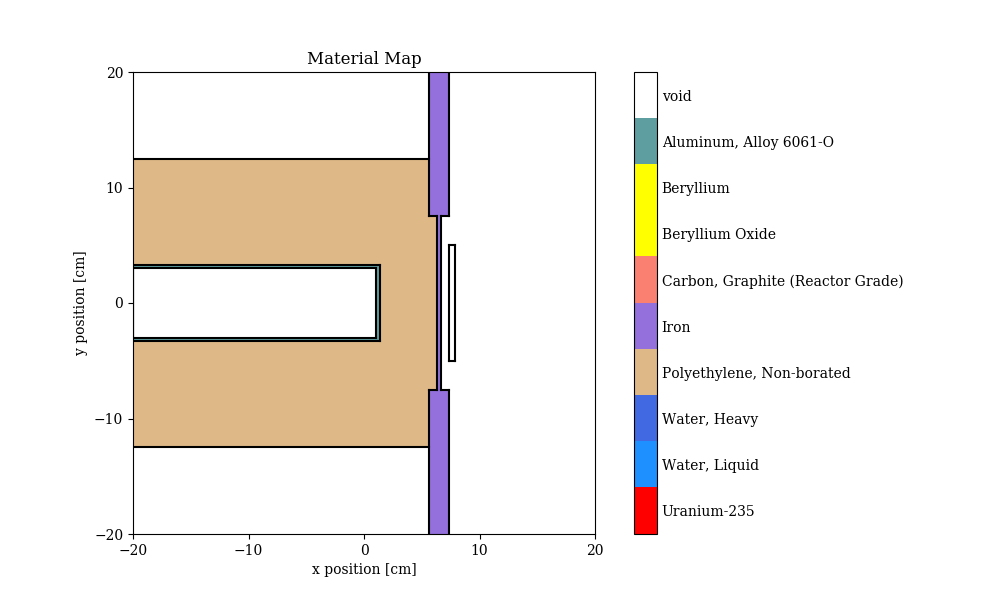
\includegraphics[trim={0.7in 0.2in 0.9in 0.45in},clip,scale=0.36]{images/material_map.png}
    \end{figure}
  \end{columns}
  \begin{itemize}
    \item Variables: location of target, moderator material (just one)
    \item The ${}^{235}\text{U}$ fission cross section is highest at thermal
          energies, but DD neutrons are produced at \tildecenter 2.45 MeV, so a
          moderator is needed
    \item I thought to myself, ``it's really too bad nobody had ever used a
          perturbed version of the transport equation to avoid needing to run
          MCNP 50 times to optimize geometry''
  \end{itemize}
\end{frame}

\begin{frame}
  \frametitle{Test Problem Construction}
  \begin{itemize}
    \item The original problem was comprised entirely of right circular
          cylinders (RCCs). Since ADVANTG requires a cartesian mesh to pass to
          Denovo, the geometry was modified to be all rectangular
          parallelepipeds (RPPs) to avoid having mesh elements with mixed
          materials.
    \item Spatial mesh has $43 \times 44 \times 44 = \text{83,248}$ elements
    \item Scalar flux has 2,081,200 values (25 energy groups)
    \item Angular flux has 266,393,600 values (128 angles)
    \item The angular forward and adjoint flux take up 4 GB of space
  \end{itemize}
\end{frame}

\begin{frame}
  \frametitle{Source and Response Location}
  \begin{columns}
    \column{0.5\textwidth}
    \begin{figure}
      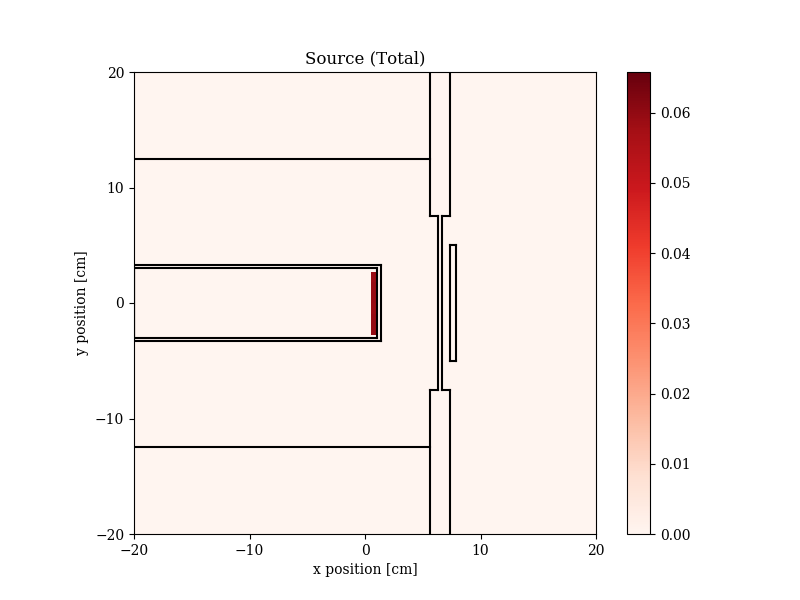
\includegraphics[trim={0.7in 0.15in 1.05in 0.4in},clip,scale=0.36]{images/source_total.png}
    \end{figure}
    \column{0.5\textwidth}
    \begin{figure}
      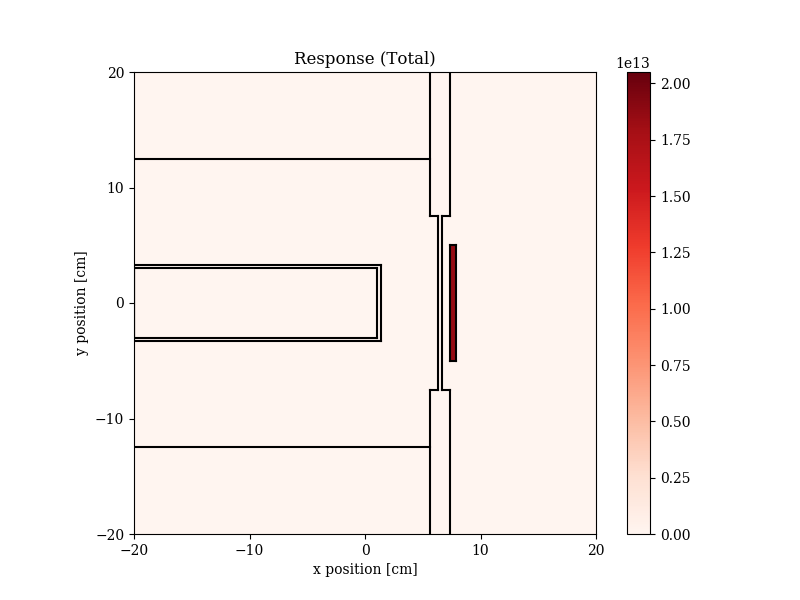
\includegraphics[trim={0.7in 0.15in 1.05in 0.4in},clip,scale=0.36]{images/response_total.png}
    \end{figure}
  \end{columns}
  \begin{itemize}
    \item Source is at the end of the vacuum tube
    \item Response is behind the thin layer of iron
  \end{itemize}
\end{frame}

\begin{frame}
  \frametitle{Source and Response Energy Spectra}
  \begin{columns}[c]
    \column{0.3\textwidth}
    \begin{itemize}
      \item Energy groups go from high to low
      \item Source is the DD fusion spectrum (\tildecenter 2.45 MeV)
      \item Response is the ${}^{235}\text{U}$ fission cross section
    \end{itemize}
    \column{0.7\textwidth}
    \begin{figure}
      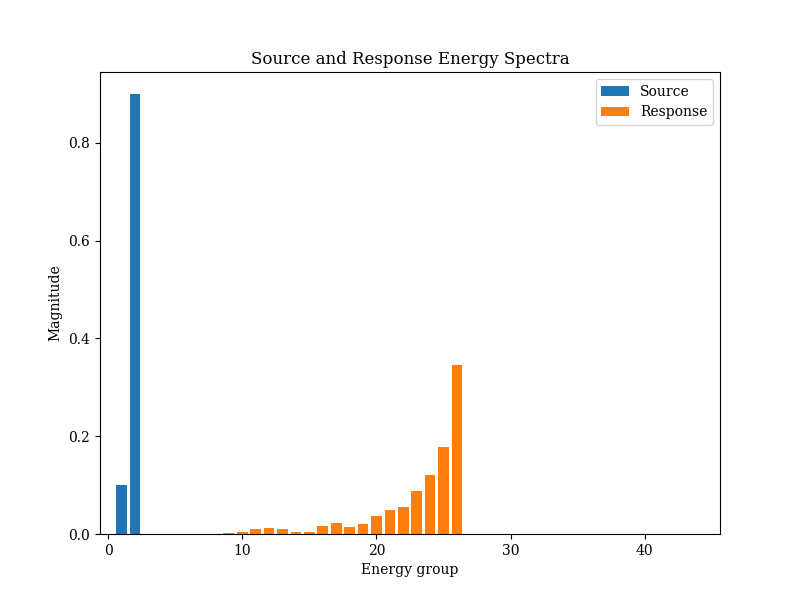
\includegraphics[trim={0.4in 0.2in 0.75in 0.4in},clip,scale=0.45]{images/spectra_lin.png}
    \end{figure}
  \end{columns}
\end{frame}

\begin{frame}
  \frametitle{Scalar Forward Flux ($\phi$)}
  \vskip-0.25in
  \begin{equation}
    \phi\left(\vec{r},E\right) = \int\psi\left(\vec{r},\hat{\Omega},E\right)d\hat{\Omega}
    %\phi = \int\psi d\hat{\Omega}
  \end{equation}
  \vskip-0.25in
  \begin{columns}
    \column{0.5\textwidth}
    \begin{figure}
      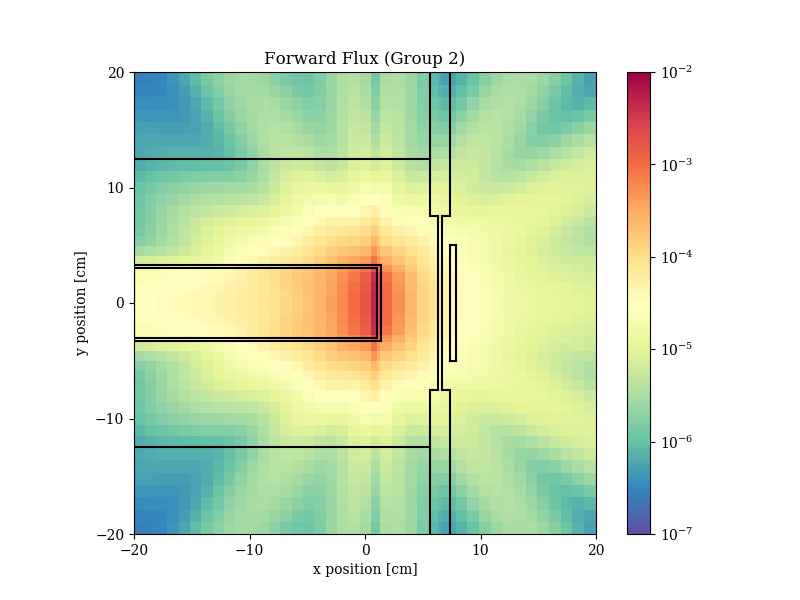
\includegraphics[trim={0.7in 0.15in 1.05in 0.4in},clip,scale=0.36]{images/scalar_flux_fwd_g02.png}
    \end{figure}
    \column{0.5\textwidth}
    \begin{figure}
      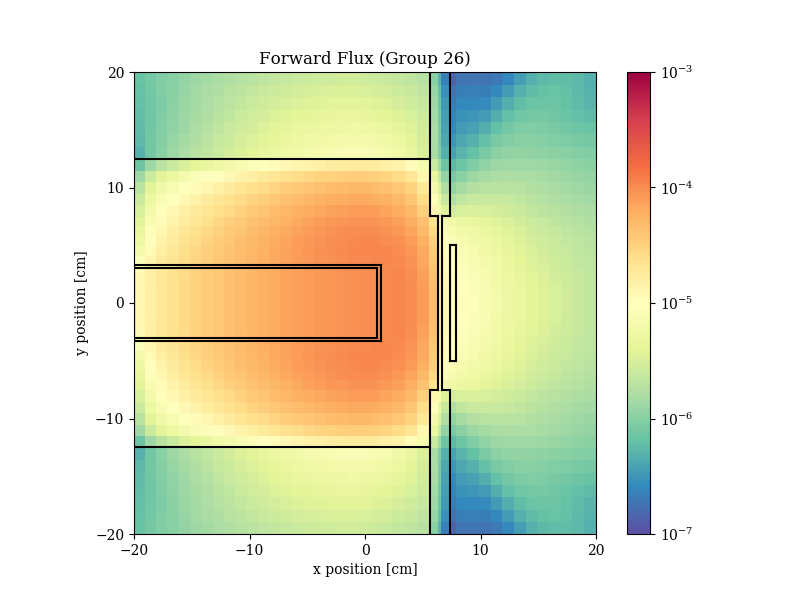
\includegraphics[trim={0.7in 0.15in 1.05in 0.4in},clip,scale=0.36]{images/scalar_flux_fwd_g26.png}
    \end{figure}
  \end{columns}
  \begin{itemize}
    \item Group 2: Highest neutron energy group in problem
    \item Group 26: Lowest neutron energy group (thermal)
    \item Ray effects clearly visible
  \end{itemize}
\end{frame}

\begin{frame}
  \frametitle{Scalar Adjoint Flux ($\phi^+$)}
  \vskip-0.25in
  \begin{equation}
    \phi^+\left(\vec{r},E\right) = \int\psi^+\left(\vec{r},\hat{\Omega},E\right)d\hat{\Omega}
    %\phi^+ = \int\psi^+d\hat{\Omega}
  \end{equation}
  \vskip-0.25in
  \begin{columns}
    \column{0.5\textwidth}
    \begin{figure}
      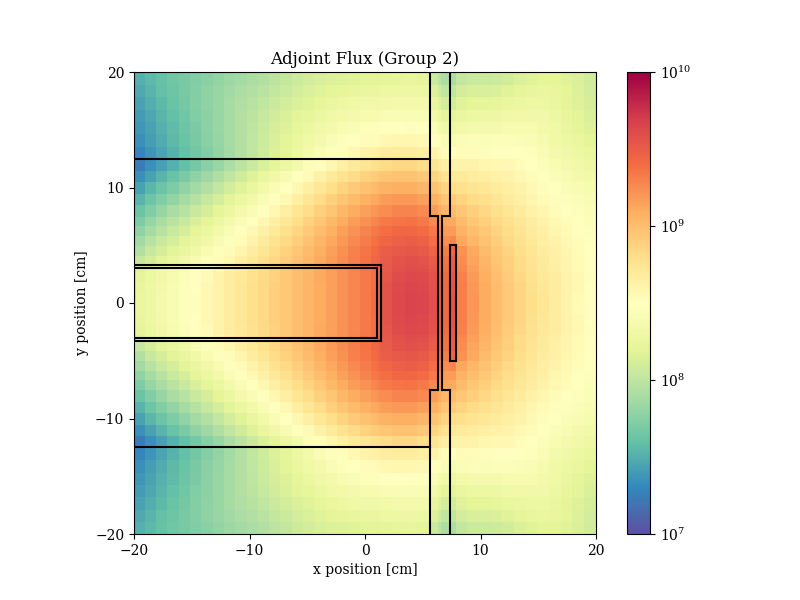
\includegraphics[trim={0.7in 0.15in 1.05in 0.4in},clip,scale=0.36]{images/scalar_flux_adj_g02.png}
    \end{figure}
    \column{0.5\textwidth}
    \begin{figure}
      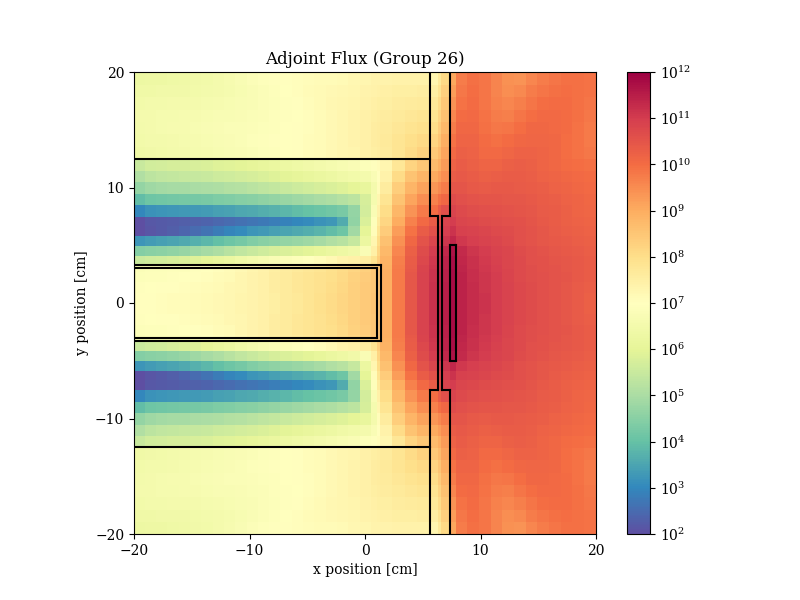
\includegraphics[trim={0.7in 0.15in 1.05in 0.4in},clip,scale=0.36]{images/scalar_flux_adj_g26.png}
    \end{figure}
  \end{columns}
  \begin{itemize}
    \item Adjoint "particles" start at the detector with a fission cross section
          spectrum (i.e. mostly thermal neutrons) and scatter upwards to higher energies
  \end{itemize}
\end{frame}

\begin{frame}
  \frametitle{Scalar Contributon Flux ($\phi_{contrib}$)}
  \vskip-0.25in
  \begin{equation}
    \phi_{contrib}\left(\vec{r},E\right) = \int\psi\left(\vec{r},\hat{\Omega},E\right)\psi^+\left(\vec{r},-\hat{\Omega},E\right)d\hat{\Omega}
    %\phi_{contrib} = \int\psi\psi^+d\hat{\Omega}
  \end{equation}
  \vskip-0.25in
  \begin{columns}
    \column{0.5\textwidth}
    \begin{figure}
      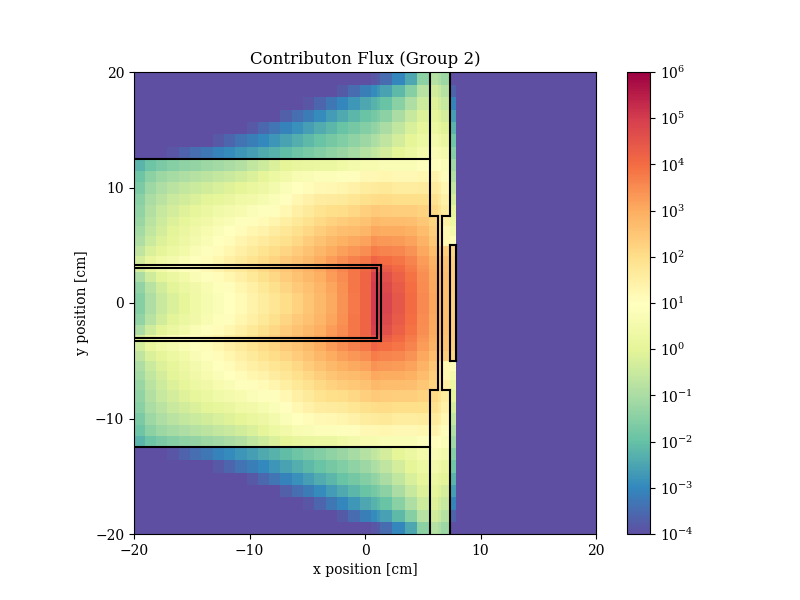
\includegraphics[trim={0.7in 0.15in 1.05in 0.4in},clip,scale=0.36]{images/scalar_flux_con_g02.png}
    \end{figure}
    \column{0.5\textwidth}
    \begin{figure}
      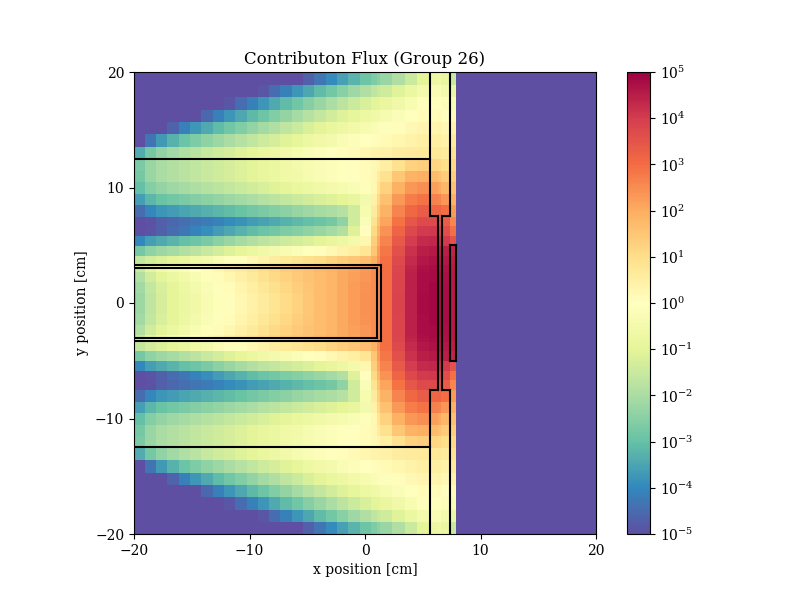
\includegraphics[trim={0.7in 0.15in 1.05in 0.4in},clip,scale=0.36]{images/scalar_flux_con_g26.png}
    \end{figure}
  \end{columns}
  \begin{itemize}
    \item Contributon shows most important paths between source and detector
    \item Note that the opposite angle must be used for the adjoint flux in
          order to calculate the contributon correctly
  \end{itemize}
\end{frame}

\begin{frame}
  \frametitle{Forward Current ($\vec{J}$)}
  \vskip-0.25in
  \begin{equation}
    \vec{J}\left(\vec{r},E\right) = \int\psi\left(\vec{r},\hat{\Omega},E\right)\hat{\Omega}d\hat{\Omega}
    %\vec{J} = \int\psi\hat{\Omega}d\hat{\Omega}
  \end{equation}
  \vskip-0.25in
  \begin{columns}
    \column{0.5\textwidth}
    \begin{figure}
      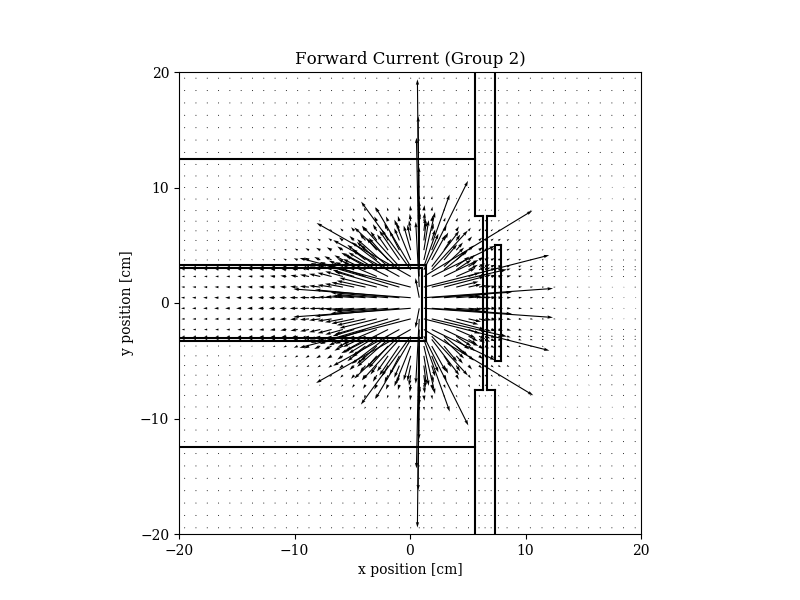
\includegraphics[trim={0.7in 0.15in 1.05in 0.4in},clip,scale=0.36]{images/current_fwd_g02.png}
    \end{figure}
    \column{0.5\textwidth}
    \begin{figure}
      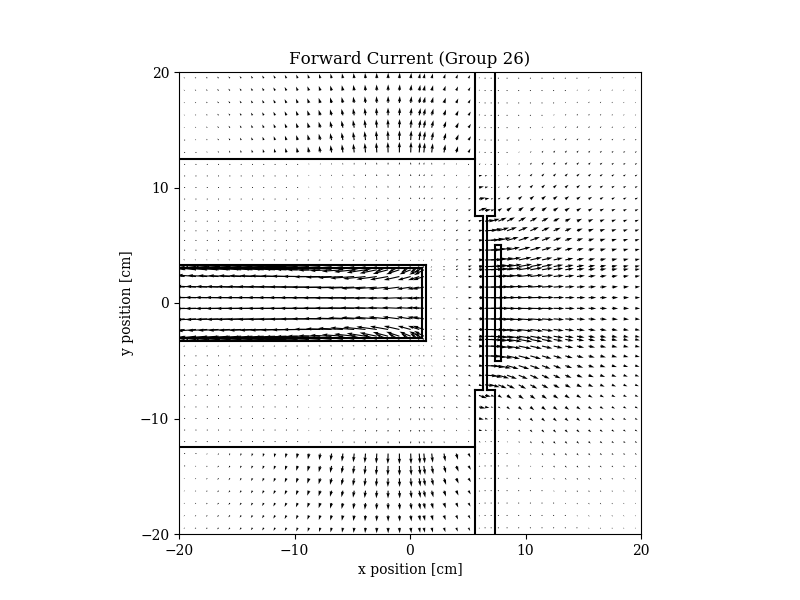
\includegraphics[trim={0.7in 0.15in 1.05in 0.4in},clip,scale=0.36]{images/current_fwd_g26.png}
    \end{figure}
  \end{columns}
  \begin{itemize}
    \item Current shows the net directionality of the flux
    \item Fast flux radiates outward from the source
    \item Thermal flux is very isotropic within the moderator region
  \end{itemize}
\end{frame}

\begin{frame}
  \frametitle{Adjoint Current ($\vec{J}^+$)}
  \vskip-0.25in
  \begin{equation}
    \vec{J}^+\left(\vec{r},E\right) = \int\psi^+\left(\vec{r},\hat{\Omega},E\right)\hat{\Omega}d\hat{\Omega}
    %\vec{J}^+ = \int\psi^+\hat{\Omega}d\hat{\Omega}
  \end{equation}
  \vskip-0.25in
  \begin{columns}
    \column{0.5\textwidth}
    \begin{figure}
      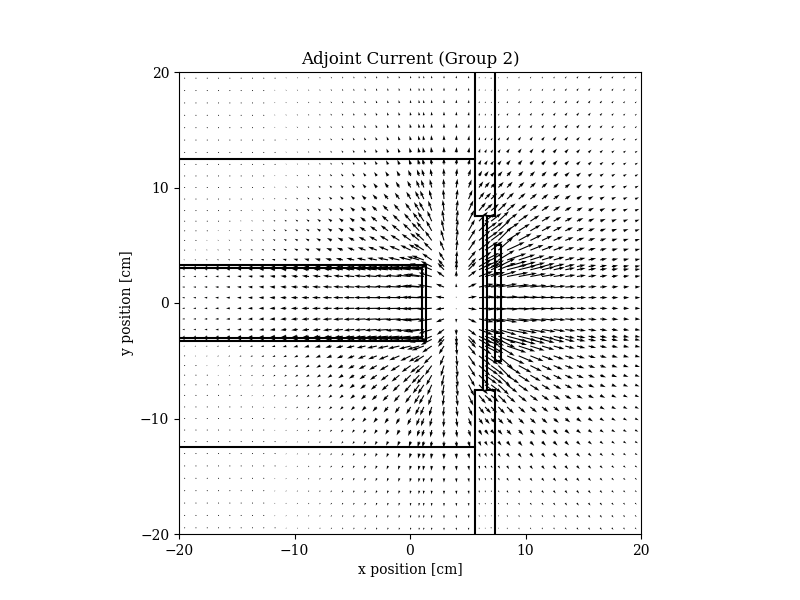
\includegraphics[trim={0.7in 0.15in 1.05in 0.4in},clip,scale=0.36]{images/current_adj_g02.png}
    \end{figure}
    \column{0.5\textwidth}
    \begin{figure}
      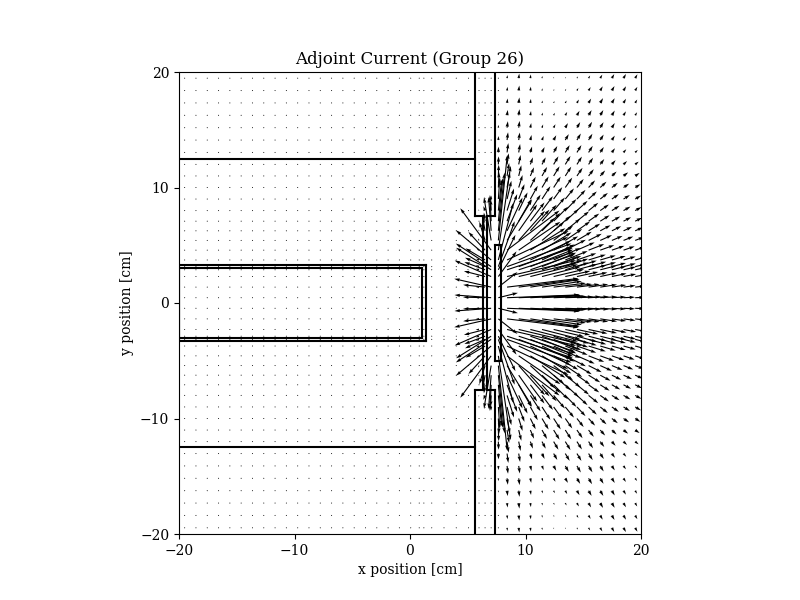
\includegraphics[trim={0.7in 0.15in 1.05in 0.4in},clip,scale=0.36]{images/current_adj_g26.png}
    \end{figure}
  \end{columns}
  \begin{itemize}
    \item Adjoint current shows the net directionality of the adjoint flux
    \item Adjoint thermal flux radiates outward from detector
    \item Adjoint fast flux radiates outward from moderator region
  \end{itemize}
\end{frame}

%\begin{frame}
%  \frametitle{Contributon Current ($\vec{J}_{contrib}$)}
%  \begin{equation}
%    \vec{J}_{contrib}\left(\vec{r},E\right)
%  \end{equation}
%  \begin{columns}
%    \column{0.5\textwidth}
%    \begin{figure}
%      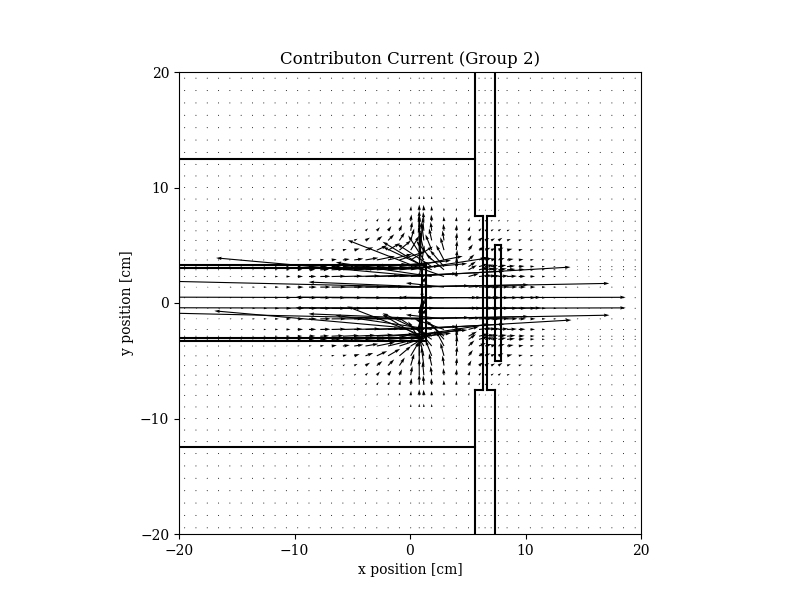
\includegraphics[trim={0.7in 0.15in 1.05in 0.4in},clip,scale=0.36]{images/current_con_g02.png}
%    \end{figure}
%    \column{0.5\textwidth}
%    \begin{figure}
%      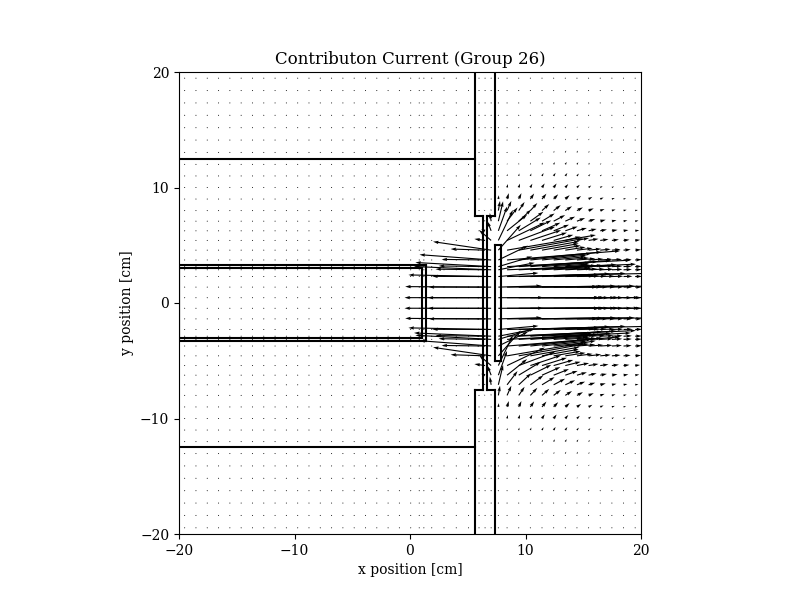
\includegraphics[trim={0.7in 0.15in 1.05in 0.4in},clip,scale=0.36]{images/current_con_g26.png}
%    \end{figure}
%  \end{columns}
%  \begin{itemize}
%    \item Contributon current
%  \end{itemize}
%\end{frame}

\begin{frame}
  \frametitle{Calculation of $\delta R$ in Test Problem}
  \vskip-0.1in
  \begin{equation*}
    \delta R = \left<\psi^+,-\delta H\psi\right>
  \end{equation*}
  \vskip-0.1in
  \begin{itemize}
    \item $\delta R$ was originally a scalar value which represented the
          perturbation in the detector response given a perturbation in the
          cross sections at some location.
    \item The definition of $\delta R$ was expanded to refer to the
          perturbation in the detector response given a perturbation in the
          cross sections at \textbf{all} locations individually.
    \item The definition of the perturbation in this test problem was replacing
          whatever material existed in each mesh element with a different
          material. This was repeated for many different materials to see the
          effect of changing to different materials in all mesh elements.
    \item Red values represent positive values of $\delta R$; blue values
          represent negative values.
  \end{itemize}
\end{frame}

\begin{frame}
  \frametitle{Perturbation in Response ($\delta R$)}
  \vskip-0.25in
  \begin{equation}
    \delta R\left(\vec{r}\right) = \iint\psi^+\left(\iint\delta\sigma_s\psi d\hat{\Omega}^\prime dE^\prime - \delta\sigma_t\psi\right)d\hat{\Omega}dE
  \end{equation}
  \vskip-0.25in
  \begin{columns}
    \column{0.5\textwidth}
    \begin{figure}
      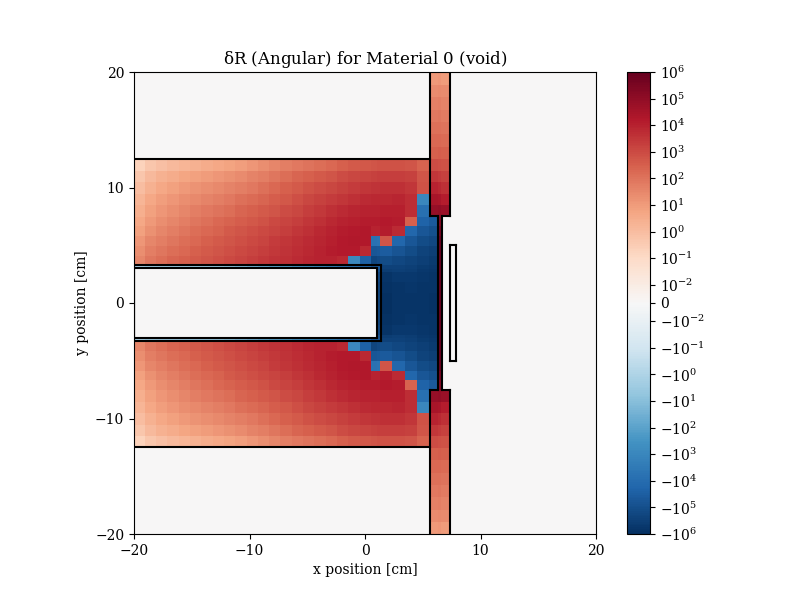
\includegraphics[trim={0.7in 0.15in 1.05in 0.4in},clip,scale=0.36]{images/dR_angular_00.png}
    \end{figure}
    \column{0.5\textwidth}
    \begin{figure}
      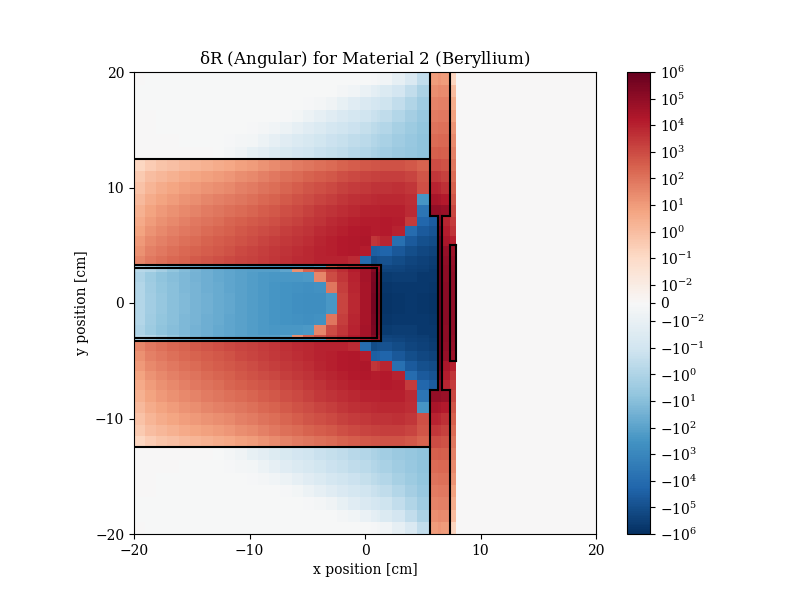
\includegraphics[trim={0.7in 0.15in 1.05in 0.4in},clip,scale=0.36]{images/dR_angular_02.png}
    \end{figure}
  \end{columns}
  \begin{itemize}
    \item Effect of replacing each mesh element with void (left) and beryllium
          (right)
    \item Anywhere the plot is red, the perturbation results in an increase in
          the response; anywhere the plot is blue, the opposite is true.
  \end{itemize}
\end{frame}

\begin{frame}
  \frametitle{Perturbation in Response ($\delta R$)}
  \vskip-0.25in
  \begin{equation*}
    \delta R\left(\vec{r}\right) = \iint\psi^+\left(\iint\delta\sigma_s\psi d\hat{\Omega}^\prime dE^\prime - \delta\sigma_t\psi\right)d\hat{\Omega}dE
  \end{equation*}
  \vskip-0.25in
  \begin{columns}
    \column{0.5\textwidth}
    \begin{figure}
      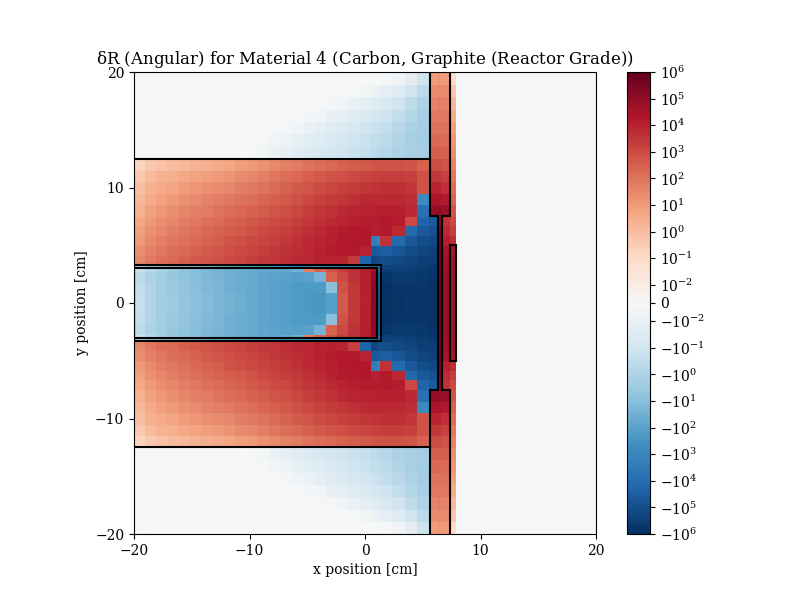
\includegraphics[trim={0.7in 0.15in 1.05in 0.4in},clip,scale=0.36]{images/dR_angular_04.png}
    \end{figure}
    \column{0.5\textwidth}
    \begin{figure}
      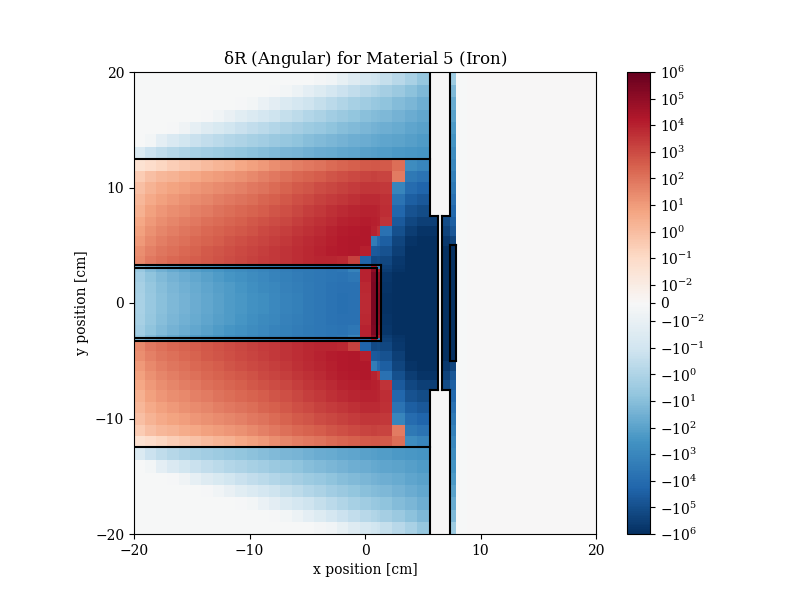
\includegraphics[trim={0.7in 0.15in 1.05in 0.4in},clip,scale=0.36]{images/dR_angular_05.png}
    \end{figure}
  \end{columns}
  \begin{itemize}
    \item Effect of replacing each mesh element with graphite (left) and iron
          (right)
    \item $\delta R$ is zero and the plot is white when the perturbation
          replaces a material with itself
  \end{itemize}
\end{frame}

\begin{frame}
  \frametitle{Perturbation in Response ($\delta R$)}
  \vskip-0.25in
  \begin{equation*}
    \delta R\left(\vec{r}\right) = \iint\psi^+\left(\iint\delta\sigma_s\psi d\hat{\Omega}^\prime dE^\prime - \delta\sigma_t\psi\right)d\hat{\Omega}dE
  \end{equation*}
  \vskip-0.25in
  \begin{columns}
    \column{0.5\textwidth}
    \begin{figure}
      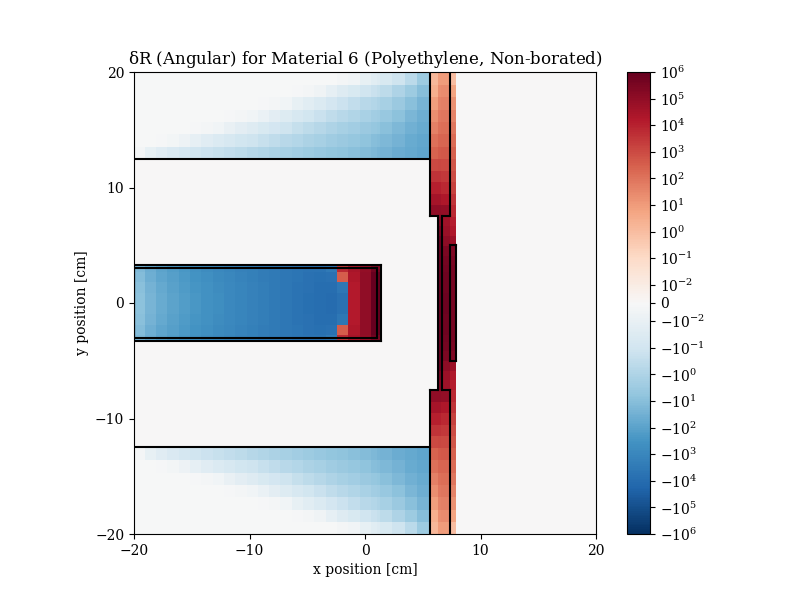
\includegraphics[trim={0.7in 0.15in 1.05in 0.4in},clip,scale=0.36]{images/dR_angular_06.png}
    \end{figure}
    \column{0.5\textwidth}
    \begin{figure}
      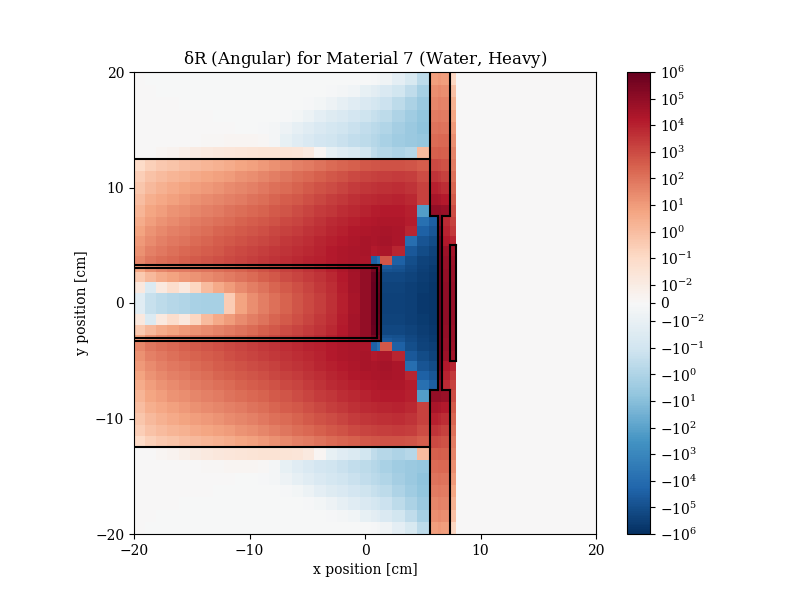
\includegraphics[trim={0.7in 0.15in 1.05in 0.4in},clip,scale=0.36]{images/dR_angular_07.png}
    \end{figure}
  \end{columns}
  \begin{itemize}
    \item Effect of replacing each mesh element with HDPE plastic (left) and
          heavy water (right)
  \end{itemize}
\end{frame}

\begin{frame}
  \frametitle{Perturbation in Response ($\delta R$)}
  \vskip-0.25in
  \begin{equation*}
    \delta R\left(\vec{r}\right) = \iint\psi^+\left(\iint\delta\sigma_s\psi d\hat{\Omega}^\prime dE^\prime - \delta\sigma_t\psi\right)d\hat{\Omega}dE
  \end{equation*}
  \vskip-0.25in
  \begin{columns}
    \column{0.5\textwidth}
    \begin{figure}
      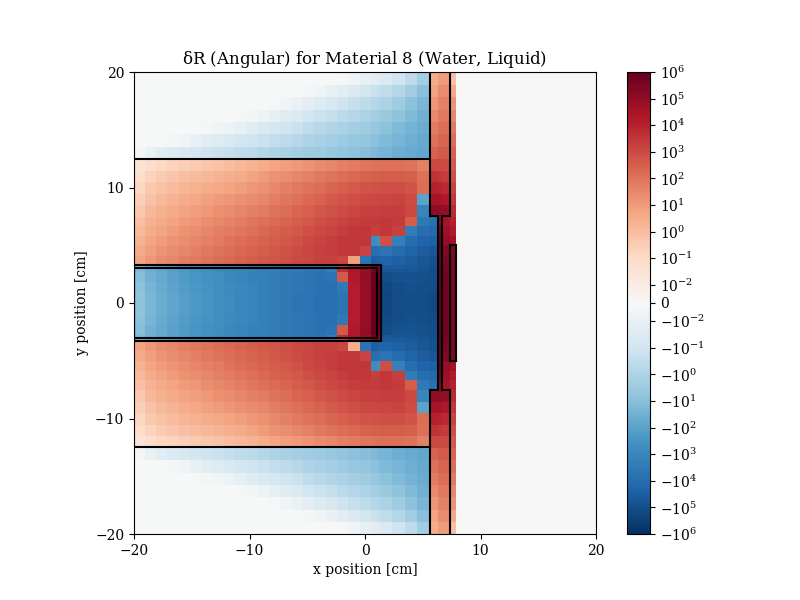
\includegraphics[trim={0.7in 0.15in 1.05in 0.4in},clip,scale=0.36]{images/dR_angular_08.png}
    \end{figure}
    \column{0.5\textwidth}
    \begin{figure}
      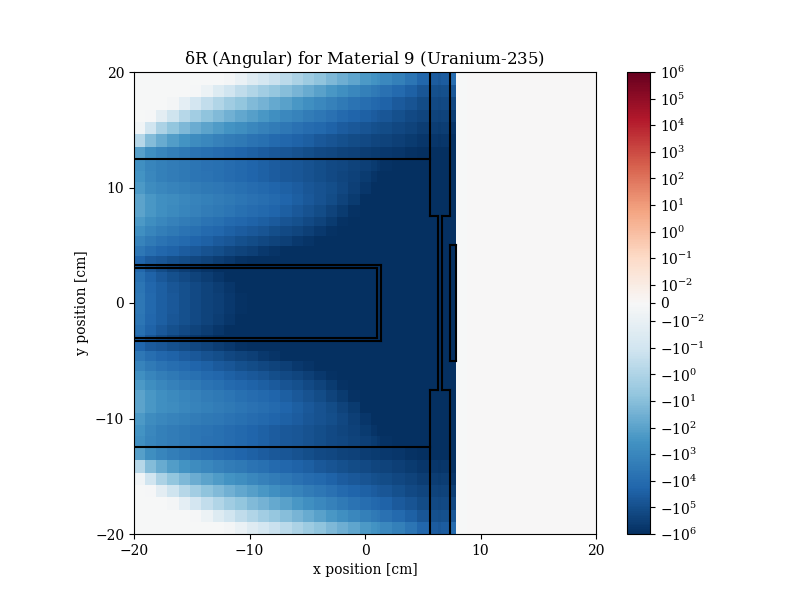
\includegraphics[trim={0.7in 0.15in 1.05in 0.4in},clip,scale=0.36]{images/dR_angular_09.png}
    \end{figure}
  \end{columns}
  \begin{itemize}
    \item Effect of replacing each mesh element with light water (left) and
          uranium-235 (right)
  \end{itemize}
\end{frame}

\begin{frame}
  \frametitle{Room for Improvement}
  \begin{itemize}
  \item The method gives the incorrect results in certain regions even when
        using the angular flux. The left-pointing current of both the forward
        and ajoint angular flux in the right-side void is zero, so the
        contributon flux in that region is zero, which means that dR in that
        region is also zero.
  \item This is clearly an incorrect result, because adding \textbf{any}
        material in that region should increase the response. This is because
        any scattering that takes place in that region can only increase the
        response, and there is no way for any interactions in that region to
        decrease the response.
  \item $\delta R$ was originally calculated using the scalar flux, not the
        angular flux, and this behavior was not seen then. The results were not
        as good in other locations in the problem, though.
  \end{itemize}
\end{frame}

% ==============================================================================
% Future work section
% ==============================================================================

\begin{frame}
  \frametitle{Future Work: Math}
  \begin{itemize}
    \item Decision space:
    \begin{itemize}
      \item What kind of changes should be allowed?
      \item What if some materials must remain fixed?
      \item What if only a certain volume of a given material is allowed to be
            used?
      \item Should mesh elements be allowed to contain multiple materials (as a
            proxy for volume fraction)?
    \end{itemize}
    \item Objective function:
    \begin{itemize}
      \item What if the overall repsonse is the sum of two responses?
      \item Or the product? Or the quotient, or some other combination?
      \item Or a simple response, but with the contraint that a different
            response must be kept below a certain threshold?
    \end{itemize}
  \end{itemize}
\end{frame}

\begin{frame}
  \frametitle{Future Work: Automation}
  \begin{itemize}
    \item The real goal is an automated system which runs transport, calculates
          $\delta R$, decides how to change the geometry, reruns transport, and
          continues until the geometry has converged to the optimal solution.
    \item It's unclear what kind of optimization algorithm would be correct to
          use. Conjugate gradient method?
  \end{itemize}
\end{frame}

\end{document}
